\subsection{BGP Routing in an Autonomous System}
\label{sec:backg}
%%%
%%% background.tex
%%%
An AS uses external BGP (eBGP) to exchange reachability information
with neighboring domains and internal BGP (iBGP) to distribute routes
inside the AS, as shown in Figure~\ref{fig:today}.  Each router
invokes the BGP decision process to select a single ``best'' route for
each destination prefix from the candidate routes learned from eBGP and iBGP.
The router combines the best BGP route with information about the
internal network topology from the Interior Gateway Protocol
(IGP) to construct a forwarding table that maps
destination prefixes to outgoing links.  Most of the flexibility and
complexity of BGP routing comes from the following three areas:

\textbf{Path selection:} A route to a destination prefix
includes attributes such as the AS path, local preference, origin
type, and multi-exit discriminator (MED).  Each router applies a
decision process~\cite{id-bgp4} that consists of a sequence of rules
that ranks the routes.  After preferring routes with highest local
preference, smallest AS path length, lowest origin type, and smallest
MED, the decision process favors eBGP-learned routes over iBGP-learned
routes.  If multiple equally-good routes remain, the router favors the
BGP route learned from the nearest border router---the {\em egress
point\/} with the smallest IGP path cost---following the common
practice of ``hot-potato'' routing.  The final tiebreak is
vendor-dependent and may depend on the age of the routes or an
arbitrary router ID.


\begin{figure}
\centering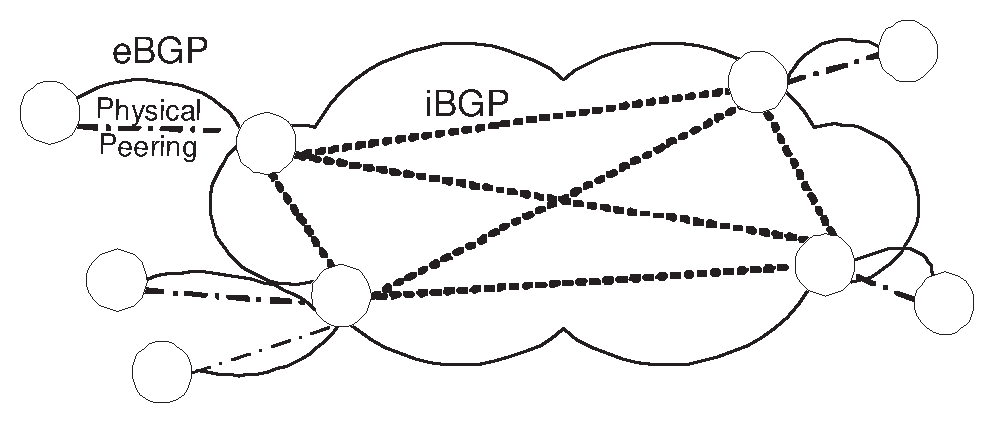
\epsfig{file=rcp/figures/today.eps, width=0.75\linewidth}
\caption[Operation of BGP routing inside an AS.]{Operation of BGP
routing inside an AS.  Most small networks use a 
``full mesh'' iBGP configuration, where every router in the AS has an
  iBGP session to every other router.} 
\label{fig:today}
\end{figure}

\textbf{Intra-AS route distribution:} Network operators can propagate
eBGP-learned routes throughout an AS in many different ways.\footnote{In
most IP backbone networks, every router needs to receive BGP routing
information to construct a complete forwarding table.  In a
Multi-Protocol Label Switching (MPLS) network, only the border routers
need to send and receive the BGP routes; the internal routers would
simply forward packets on label-switched paths from the ingress router
to the egress point.}  Small networks typically have a ``full mesh'' of
iBGP sessions, as shown in Figure~\ref{fig:today}.  To avoid the $n^2$
scaling problem, a large AS may have a more complex iBGP
topology.
%, where each edge corresponds to an iBGP session between two
%routers.  
For example, although a router does not normally forward
iBGP-learned routes to its other iBGP neighbors, it can be configured
as a {\em route reflector\/}, which forwards routes learned from one
route-reflector client to another.  A router forwards only its {\em
best\/} route to its iBGP neighbors, making the choices available at one
router depend on decisions made by its iBGP neighbors, as shown in
Figure~\ref{fig:rr}.
\begin{figure}
\centering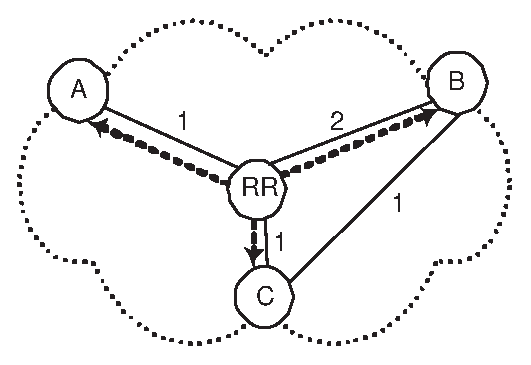
\epsfig{file=rcp/figures/rr.eps, width=0.4\linewidth}
\caption[An example route reflector topology that does not emulate
full-mesh iBGP.]{An example of where iBGP with route reflection does not
emulate 
full-mesh iBGP; numbers represent IGP path costs, and arrows
indicate an iBGP session from a route reflector to its client.  In a
full-mesh, router $C$ would prefer routes learned from $B$ over routes
learned from $A$ because its IGP path cost to $B$ is smaller.  However,
in the example shown, $RR$ prefers $A$, and, thus, $C$ must also select $A$.}
\label{fig:rr}
\end{figure}

\textbf{Routing policy:}
Network operators influence path selection by configuring import and
export policies on the eBGP sessions to neighboring domains.  An {\em
  import\/} policy 
filters unwanted routes and manipulates the attributes of the
remaining routes; for example, the policy could assign a small local
preference to routes learned from one neighbor to make these routes
less attractive than routes learned from other neighbors.  After
selecting a single best route, the router applies an {\em export\/}
policy to manipulate the attributes and decide whether to propagate
the route to a neighbor.  For example, a router may be configured to
export routes learned from a private peer to a customer but not to
another private peer.

